\section{Modelling electron correlations in energy bands}\label{sec:intro}

The interactions between the electrons in a solid give rise to effects that arise specifically due to the many-body nature of the system.
These strong electron correlations are often studied in the context of the Hubbard model.
The latter goes beyond the periodic ionic potential perturbation to the free electron gas or tight binding approaches, which lead to band theory, by adding an interaction term to the tight binding Hamiltonian. 
Using it, we can make predictions about properties of a strongly correlated system, namely magnetic and superconducting behavior, and metal-insulator transitions.

Appearing in 1963 as one of the first attempts to include electron interaction effects in a quantum mechanical description of a solid, the Hubbard model was originally introduced to explain the behavior of the electrons in the narrow, partially filled $d-$bands of transition metals \cite{hubbard_electron_1963}.
Correlation phenomena due to the Coulomb repulsion between the electrons in these bands lead to a behavior reminiscent of the atomic picture of a solid.
In fact, the model may simply be regarded as a minimal model of interacting electrons in an energy band of a solid, where only on-site interactions penalizing double occupancy are considered.
We have come a long way since the introduction of the Hubbard model and it is now arguably as paradigm-defining in many-body theory as the Ising model in statistical physics \cite{fazekas_lecture_1999, mahan_many-particle_2000, altland_condensed_2010}.
Although it was initially applied to transition metal monoxides like \chem{FeO}, \chem{NiO}, and \chem{CoO}, which are antiferromagnetic insulators (and not metallic, as was initially thought)\footnote{They were predicted to be metals by band theory until they were found not to behave like metals empirically.}, it gives insight on insulating, magnetic, and even superconducting phases arising due to the effect of electron interactions in a variety of quantum systems.
\begin{figure}[H]
	\centering
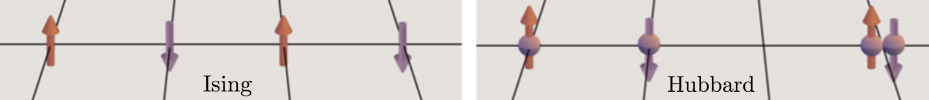
\includegraphics[scale=0.4]{Hubbard/IsingVsHubbard.png}
	\caption[Graphical comparison between the Ising and the Hubbard models.]{Unlike the Ising model, where either an up or a down spin live at each site, in the Hubbard model, there are four possible states at each site: a "hole" (absence of an electron), either an up spin electron or a down spin electron, or two electrons of opposite spins.
	The idea behind the model is to consider that the electrons interact, repelling each other (or attracting, in the case of superconductivity), only when they are on the same site (taken from \cite{hayes_hip-hop_2009}).}
	\label{fig:IsingVsHubbard}
\end{figure}

Fig.(\ref{fig:IsingVsHubbard}) is only a simplified view presented for comparison with a classical model of magnetism.
The Hubbard Hamiltonian acts on electron wave functions centered on the sites of a lattice, leading to simultaneous charge and spin fluctuations. 
Ultimately, we wish to determine, or at least approximate, the wave function describing the full electronic system. 
Due to the many-body effects of electron correlations, this wave function is not a simple combination of products of one electron wave functions (a Slater determinant), as in the interaction-free case, or for nearly free electrons.

In the 1950's, the community was working on a theory of correlation effects in the free electron gas \cite{bohm_collective_1953, gell-mann_correlation_1957, sawada_correlation_1957, hubbard_description_1958, hubbard_description_1958_2, nozieres_electron_1958}, which motivated Hubbard to devise a simple model for the (at the time) seemingly intractable problem of interacting electrons in a band.
It became popular because it is generally realistic, yet relatively amenable to both analytical and numerical computations after some controlled approximations are introduced.
Notably, it has been shown to be very relevant in the description of Mott insulators, and high $T_c$  superconductors\footnote{In this context, $T_c$ is the critical temperature associated with the transition to a superconducting phase.}.
In fact, the Hubbard model has found many applications, describing successfully a variety of quantum systems \cite{editorial_hubbard_2013}; nonetheless, even the simplified picture it offers is in general difficult to approach analytically.
There exists an exact solution in one dimension via Bethe ansatz \cite{lieb_absence_1968}, however the more general higher dimensional case is often solved numerically.
An example of particular relevance for this work is the study carried out by Hirsch \cite{hirsch_two-dimensional_1985}.
In the following chapters, we will discuss how to simulate the Hubbard model using a numerical approach that is based on this seminal paper, and essentially follows the ideas introduced in it.